\documentclass[border=0.2cm, convert={density=600}]{standalone}
 
% Required packages and libraries
\usepackage{tikz}
\usetikzlibrary{shapes, positioning, arrows.meta, calc}

% custom styles
\tikzset{
  parser/.style={
    rectangle,
    rounded corners,
    draw=black, very thick,
    minimum height=2em,
    inner sep=2pt,
    text centered,
    rectangle split,
    rectangle split draw splits=false,
    rectangle split parts=2,
    draw=black
  },
  arrow/.style={
    draw=black,
    thick,
    ->,
    >=stealth
  }
}

% custom dot symbol (bigger than \cdot but smaller than \bullet)
\makeatletter
\newcommand*\dotp{\mathpalette\dotp@{.5}}
\newcommand*\dotp@[2]{\mathbin{\vcenter{\hbox{\scalebox{#2}{$\m@th#1\bullet$}}}}}
\makeatother
 
\begin{document}
 
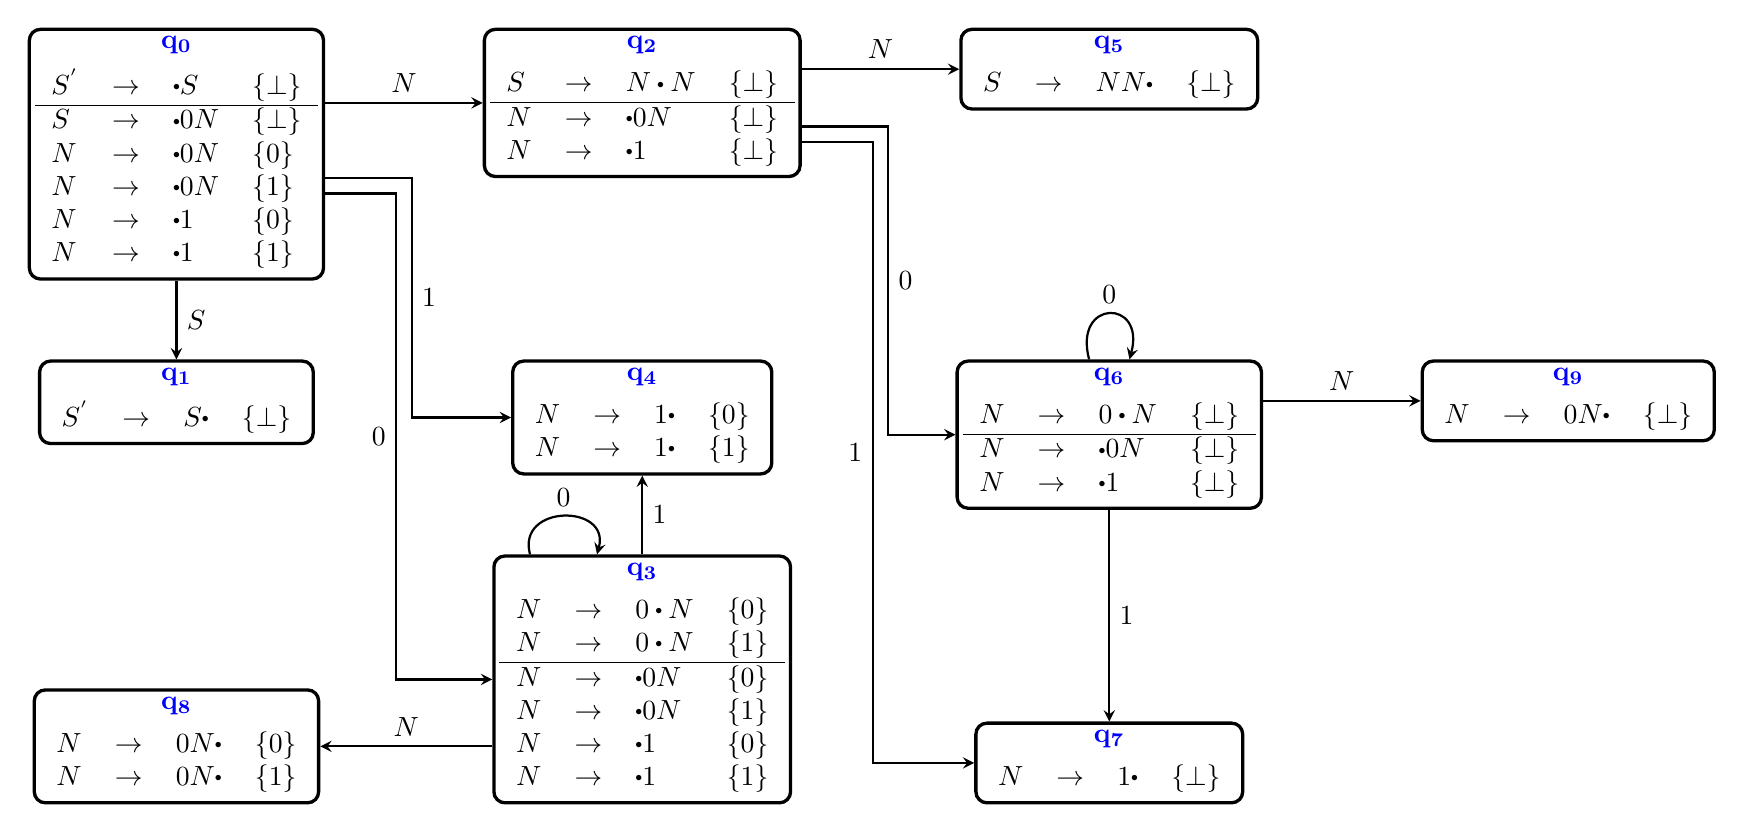
\begin{tikzpicture}
% LR(1) Parser
% Grammar:
%	(0) S' → S
%	(1) S → NN
%	(2) N → 0N
%	(3) N → 1

% nodes
\node[parser] (q0)
{ $\mathbf{\color{blue} q_{0}}$
  \nodepart{second}
  \begin{tabular}{llll}
     $S^{'}$ & $\rightarrow$ & $\dotp S$  & $\lbrace \bot \rbrace$\\
     \hline
     $S$     & $\rightarrow$ & $\dotp 0N$ & $\lbrace \bot \rbrace$\\
     $N$     & $\rightarrow$ & $\dotp 0N$ & $\lbrace 0 \rbrace$\\
     $N$     & $\rightarrow$ & $\dotp 0N$ & $\lbrace 1 \rbrace$\\
     $N$     & $\rightarrow$ & $\dotp 1$  & $\lbrace 0 \rbrace$\\
     $N$     & $\rightarrow$ & $\dotp 1$  & $\lbrace 1 \rbrace$\\
  \end{tabular}
};

\node[parser, below = 1cm of q0] (q1)
{ $\mathbf{\color{blue} q_{1}}$
  \nodepart{second}
  \begin{tabular}{llll}
     $S^{'}$ & $\rightarrow$ & $S\dotp$ & $\lbrace \bot \rbrace$\\
  \end{tabular}
};

\node[parser, right = 2cm of q0.north east, anchor=north west] (q2)
{ $\mathbf{\color{blue} q_{2}}$
  \nodepart{second}
  \begin{tabular}{llll}
     $S$ & $\rightarrow$ & $N \dotp N$ & $\lbrace \bot \rbrace$\\
     \hline
     $N$ & $\rightarrow$ & $\dotp 0 N$ & $\lbrace \bot \rbrace$\\
     $N$ & $\rightarrow$ & $\dotp 1$   & $\lbrace \bot \rbrace$\\
  \end{tabular}
};

\node[parser, anchor=north] (q4) at (q1.north -| q2.south)
{ $\mathbf{\color{blue} q_{4}}$
  \nodepart{second}
  \begin{tabular}{llll}
     $N$ & $\rightarrow$ & $1 \dotp$ & $\lbrace 0 \rbrace$\\
     $N$ & $\rightarrow$ & $1 \dotp$ & $\lbrace 1 \rbrace$\\
  \end{tabular}
};

\node[parser, below = 1cm of q4] (q3)
{ $\mathbf{\color{blue} q_{3}}$
  \nodepart{second}
  \begin{tabular}{llll}
     $N$ & $\rightarrow$ & $0 \dotp N$ & $\lbrace 0 \rbrace$\\
     $N$ & $\rightarrow$ & $0 \dotp N$ & $\lbrace 1 \rbrace$\\
     \hline
     $N$ & $\rightarrow$ & $\dotp 0 N$ & $\lbrace 0 \rbrace$\\
     $N$ & $\rightarrow$ & $\dotp 0 N$ & $\lbrace 1 \rbrace$\\
     $N$ & $\rightarrow$ & $\dotp 1$   & $\lbrace 0 \rbrace$\\
     $N$ & $\rightarrow$ & $\dotp 1$   & $\lbrace 1\rbrace$\\
  \end{tabular}
};

\node[parser, right = 2cm of q2.north east, anchor=north west] (q5)
{ $\mathbf{\color{blue} q_{5}}$
  \nodepart{second}
  \begin{tabular}{llll}
     $S$ & $\rightarrow$ & $N N \dotp$ & $\lbrace \bot \rbrace$\\
  \end{tabular}
};

\node[parser, anchor=north] (q6) at (q4.north -| q5.south)
{ $\mathbf{\color{blue} q_{6}}$
  \nodepart{second}
  \begin{tabular}{llll}
     $N$ & $\rightarrow$ & $0 \dotp N$ & $\lbrace \bot \rbrace$\\
     \hline
     $N$ & $\rightarrow$ & $\dotp 0 N$ & $\lbrace \bot \rbrace$\\
     $N$ & $\rightarrow$ & $\dotp 1$   & $\lbrace \bot \rbrace$\\
  \end{tabular}
};

\node[parser, anchor=south] (q7) at (q3.south -| q6.south)
{ $\mathbf{\color{blue} q_{7}}$
  \nodepart{second}
  \begin{tabular}{llll}
     $N$ & $\rightarrow$ & $1 \dotp$ & $\lbrace \bot \rbrace$\\
  \end{tabular}
};

\node[parser, anchor=south] (q8) at (q3.south -| q1.south)
{ $\mathbf{\color{blue} q_{8}}$
  \nodepart{second}
  \begin{tabular}{llll}
     $N$ & $\rightarrow$ & $0 N \dotp$ & $\lbrace 0 \rbrace$\\
     $N$ & $\rightarrow$ & $0 N \dotp$ & $\lbrace 1 \rbrace$\\
  \end{tabular}
};

\node[parser, right = 2cm of q6.north east, anchor=north west] (q9)
{ $\mathbf{\color{blue} q_{9}}$
  \nodepart{second}
  \begin{tabular}{llll}
     $N$ & $\rightarrow$ & $0 N \dotp$ & $\lbrace \bot \rbrace$\\
  \end{tabular}
};

% edges

%% q0
\draw [arrow] (q0.south) -- node[anchor=west]{$S$} (q1.north);
\draw [arrow] (q0.east |- q2.west) -- node[anchor=south]{$N$} (q2.west);

\coordinate[right=0.9cm of q0.east, yshift=-5mm] (h03);
\draw [arrow] (q0.east |- h03) -- (h03) -- node[left]{$0$} (h03 |- q3.west) -- (q3.west);

\coordinate[right=1.1cm of q0.east, yshift=-3mm] (h04);
\draw [arrow] (q0.east |- h04) -- (h04) -- node[right]{$1$} (h04 |- q4.west) -- (q4.west);

%% q2
\draw [arrow] (q2.east |- q5.west) -- node[anchor=south]{$N$} (q5.west);

\coordinate[right=0.9cm of q2.east, yshift=-5mm] (h27);
\draw [arrow] (q2.east |- h27) -- (h27) -- node[left]{$1$} (h27 |- q7.west) -- (q7.west);

\coordinate[right=1.1cm of q2.east, yshift=-3mm] (h26);
\draw [arrow] (q2.east |- h26) -- (h26) -- node[right]{$0$} (h26 |- q6.west) -- (q6.west);

%% q3
\path [arrow, every loop/.style={min distance=3mm,looseness=2}] (q3) edge[loop above, transform canvas={xshift=-10mm}] node[anchor=south]{$0$} ();
\draw [arrow] (q3.west |- q8.east) -- node[anchor=south]{$N$} (q8.east);
\draw [arrow] (q3.north) -- node[anchor=west]{$1$} (q4.south);

%% q6
\path [arrow, every loop/.style={min distance=5mm,looseness=4}] (q6) edge[loop above] node[anchor=south]{$0$} ();
\draw [arrow] (q6.south) -- node[anchor=west]{$1$} (q7.north);
\draw [arrow] (q6.east |- q9.west) -- node[anchor=south]{$N$} (q9.west);
\end{tikzpicture}
 
\end{document}
